\section{Fondements théoriques de l’automatisation des infrastructures}

\subsection{Évolution historique}

La gestion des systèmes d’information a connu une évolution rapide, marquée par plusieurs transformations majeures. Elle est passée de l’administration manuelle des serveurs physiques, où chaque déploiement nécessitait des opérations répétitives et susceptibles d’erreurs, à l’émergence des datacenters virtualisés et du Cloud Computing. Cette progression a été motivée par la recherche d’une meilleure agilité opérationnelle et par la nécessité de réduire les coûts d’exploitation.

La complexification des environnements informatiques a conduit à la formalisation de pratiques visant à automatiser la création, la configuration et la supervision des ressources. C’est dans ce contexte qu’a émergé le paradigme de l’Infrastructure as Code, qui constitue aujourd’hui un socle incontournable des démarches de modernisation.

\subsection{Approche DevOps}

Le développement des infrastructures modernes s’inscrit dans une démarche DevOps, qui associe les équipes de développement et d’exploitation dans une collaboration continue. Cette approche vise à réduire les cycles de livraison, améliorer la qualité logicielle et favoriser l’automatisation des processus. Elle s’appuie sur une culture de responsabilisation partagée, une intégration continue et une surveillance permanente des systèmes. DevOps contribue ainsi à faire converger les objectifs techniques et organisationnels, en alignant la production logicielle et les opérations.
\begin{figure} [H]
	\centering
	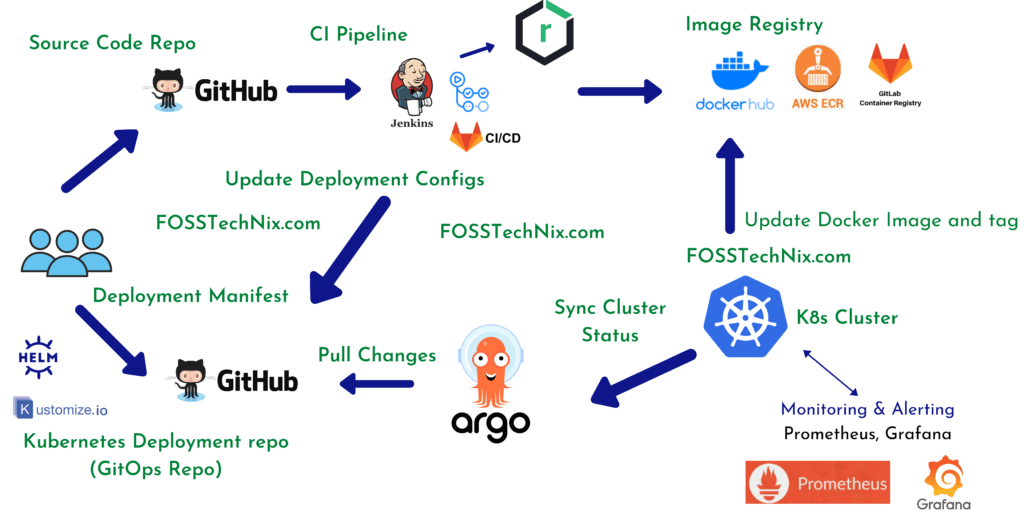
\includegraphics[width=.5\textwidth]{figures/Devops.png}
	\caption{Taches de DevOps}
	\label{fig:Taches de DevOps}
\end{figure}
\subsection{Modèles conceptuels}

L’Infrastructure as Code (IaC) désigne l’ensemble des méthodes et outils permettant de décrire l’état souhaité d’une infrastructure sous forme de fichiers de configuration versionnés et exécutables. Deux modèles se distinguent généralement : le modèle impératif, dans lequel l’utilisateur décrit la séquence exacte des opérations, et le modèle déclaratif, qui se concentre sur la définition de l’état final visé en laissant au moteur d’exécution la responsabilité d’y converger.

\subsection{Approche GitOps}

En prolongement de l’IaC, l’approche GitOps propose de faire du système de gestion de version la source unique de vérité pour la configuration et le déploiement applicatif. Elle se caractérise par un processus de déploiement automatisé, piloté par des agents qui observent l’état déclaré dans les dépôts et appliquent les modifications nécessaires aux environnements. Cette méthode garantit une traçabilité complète des évolutions, facilite le retour en arrière et renforce la cohérence entre les différents environnements. GitOps s’intègre naturellement avec les pipelines CI/CD, qui orchestrent la construction, les tests et la mise en production de façon systématique.

\section{Conteneurisation et orchestration}

\subsection{Principes de la conteneurisation}

La conteneurisation a constitué une rupture technologique majeure en introduisant une isolation légère des environnements d’exécution, en comparaison avec les machines virtuelles traditionnelles. Chaque conteneur encapsule l’application et ses dépendances, assurant ainsi une portabilité élevée et une reproductibilité des exécutions sur différents environnements.

Parmi les bénéfices les plus fréquemment identifiés figurent la réduction de la charge système, l’optimisation des coûts d’infrastructure, l’accélération des cycles de déploiement et une meilleure isolation des processus.

\subsection{Orchestration des conteneurs}

Pour coordonner ces conteneurs à grande échelle, des plateformes d’orchestration ont été développées. Kubernetes s’est progressivement imposé comme la solution de référence, grâce à sa capacité à automatiser le placement des workloads, l’ajustement dynamique des ressources, la relance des conteneurs défaillants et la gestion centralisée des configurations ainsi que des secrets. Ces fonctionnalités favorisent l’exploitation efficace d’environnements complexes et distribués.

\subsection{Patterns d’architecture cloud-native}

La conteneurisation et l’orchestration encouragent l’adoption de modèles applicatifs dits \emph{cloud-native}. Ces architectures reposent notamment sur le découpage en microservices, la scalabilité horizontale, la résilience par la redondance et le découplage entre l’infrastructure et les applications. Ces principes sont aujourd’hui largement adoptés par les entreprises souhaitant moderniser leurs systèmes d’information.

\section{Approches de supervision et d’observabilité}

\subsection{Enjeux de l’observabilité}

Dans des environnements distribués et dynamiques, l’observabilité est un facteur déterminant de fiabilité et de performance. Elle va au-delà de la supervision traditionnelle en visant une compréhension globale et en temps réel des comportements des systèmes. Cette démarche repose sur trois piliers essentiels : les métriques, qui mesurent l’état et les performances ; les logs, qui conservent l’historique des événements ; et les traces distribuées, qui permettent de suivre le parcours des requêtes au sein de l’architecture.

\subsection{Outils et standards de référence}

Différentes solutions se sont imposées comme standards de fait dans le domaine. Prometheus est souvent privilégié pour la collecte des métriques et la génération d’alertes, tandis que Grafana assure leur visualisation et leur suivi en temps réel. Elastic Stack ou Loki sont fréquemment utilisés pour l’agrégation et l’analyse des logs, et des outils tels que Jaeger et OpenTelemetry facilitent le traçage distribué. L’adoption de protocoles ouverts et d’API standardisées favorise leur intégration avec les plateformes d’orchestration.

\section{Sécurité des infrastructures automatisées}

\subsection{Principes de sécurité}

La sécurisation des infrastructures automatisées s’appuie sur le principe de \emph{Security by Design}, qui préconise l’intégration des mesures de protection dès les phases initiales de conception. Le modèle \emph{Zero Trust}, largement diffusé, repose notamment sur l’absence de confiance implicite accordée à un composant, l'identification, l’authentification et l’autorisation systématiques de chaque requête ainsi que la limitation des privilèges au strict nécessaire. Ces approches sont particulièrement adaptées aux environnements hybrides et multi-clouds.

\subsection{Gestion des secrets et des accès}

La gestion centralisée des secrets constitue une pratique essentielle pour sécuriser les identifiants, certificats et autres éléments sensibles. Elle repose sur le stockage chiffré, la rotation périodique des clés et la traçabilité des accès. Des outils spécialisés, tels que Vault, apportent des solutions robustes et éprouvées pour répondre à ces exigences.

\subsection{Sécurité périmétrique et segmentation}

La protection des infrastructures repose également sur des dispositifs périmétriques tels que les pare-feu, les listes de contrôle d’accès et la segmentation réseau. Ces mécanismes permettent de limiter la surface d’exposition, de cloisonner les environnements et de renforcer la résilience face aux attaques latérales. La mise en œuvre de politiques de filtrage strictes et le principe du moindre privilège complètent ces mesures pour réduire les risques d’intrusion.

\section{Comparaison des approches et des solutions existantes}

\subsection{Provisioning et configuration}

Différents outils se distinguent dans le domaine de la gestion automatisée des infrastructures. Terraform et CloudFormation privilégient une approche déclarative du provisioning, facilitant la reproductibilité des déploiements, tandis qu’Ansible et Chef se concentrent sur la configuration et l’orchestration logicielle. La flexibilité de Terraform dans les environnements hybrides et multi-clouds, ainsi que la simplicité d’Ansible pour la configuration idempotente, sont régulièrement mises en avant.

\subsection{Déploiement et synchronisation}

Le déploiement et la synchronisation des configurations s’inscrivent dans les pratiques GitOps, qui renforcent la traçabilité et la cohérence entre les environnements. Argo CD se démarque par une interface graphique aboutie et une intégration poussée avec Kubernetes, tandis que Flux privilégie une approche minimaliste fondée sur des mécanismes de synchronisation automatisés. Ces outils contribuent à standardiser les processus de livraison et à réduire les écarts de configuration.

\subsection{Limites identifiées}

Malgré leurs atouts, ces approches présentent certaines contraintes, parmi lesquelles une complexité opérationnelle accrue, la nécessité d’une montée en compétences significative des équipes et des risques liés à la sécurité si les configurations ne sont pas maîtrisées. Ces limites appellent la définition de processus rigoureux et l’automatisation des contrôles.